%(BEGIN_QUESTION)
% Copyright 2006, Tony R. Kuphaldt, released under the Creative Commons Attribution License (v 1.0)
% This means you may do almost anything with this work of mine, so long as you give me proper credit

Anta at en konstant strømningsrate på 20 gallon per minutt går inn i beholderen gjennom røret. Tegn denne konstante strømningen over tid, og tegn også det akkumulerte væskevolumet i beholderen over tid:

$$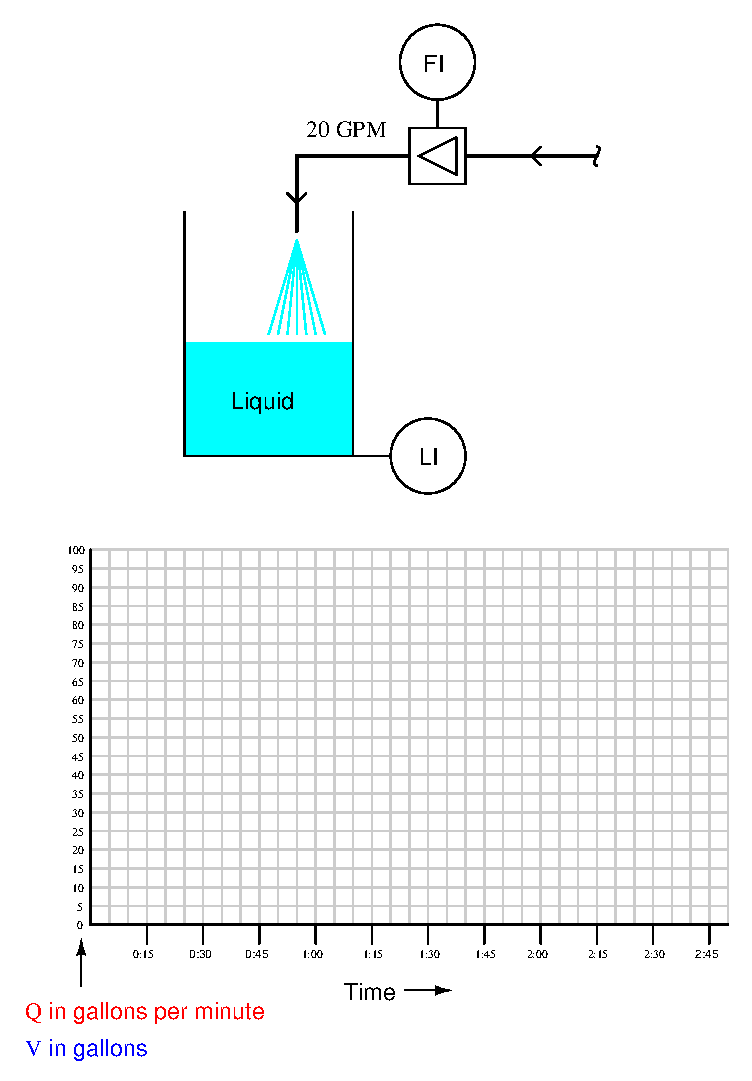
\includegraphics[width=15.5cm]{i01579x01.eps}$$

Anta at beholderen er helt tom når væsken begynner å strømme ved starttidspunktet (0:00). Merk at tidsenheten på grafens horisontale akse er minutter:sekunder, ikke timer:minutter. Forklar også hvorfor antakelsen om tom beholder ved 0:00 er viktig for å kunne forutsi totalt lagret volum i beholderen.

\filbreak

Beregn akkumulert væskevolum ved følgende tidspunkter:

\begin{itemize}
\item{} Tid = 1:00; Volum = \underbar{\hskip 50pt}
\vskip 5pt
\item{} Tid = 1:30; Volum = \underbar{\hskip 50pt}
\vskip 5pt
\item{} Tid = 2:00; Volum = \underbar{\hskip 50pt}
\vskip 5pt
\item{} Tid = 2:30; Volum = \underbar{\hskip 50pt}
\vskip 5pt
\item{} Tid = 2:45; Volum = \underbar{\hskip 50pt}
\end{itemize} 

\underbar{file i01579}
%(END_QUESTION)





%(BEGIN_ANSWER)

$$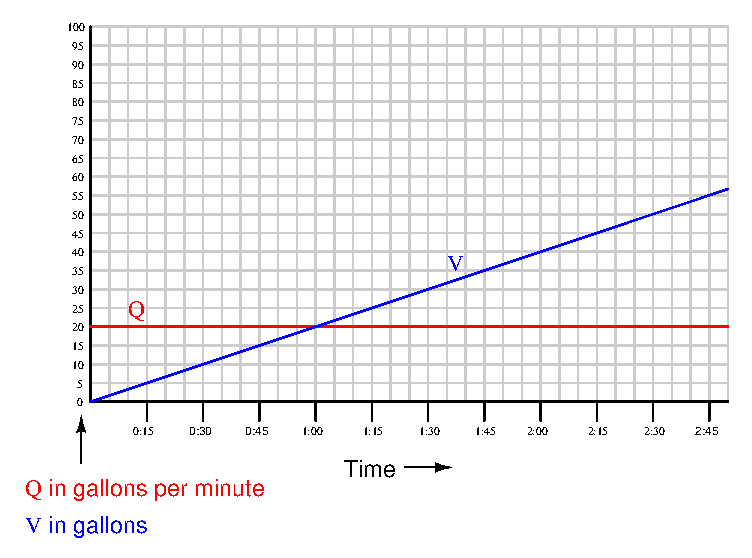
\includegraphics[width=15.5cm]{i01579x02.eps}$$

Jeg lar deg forklare hvorfor antakelsen om en tom beholder ved start er viktig!

\begin{itemize}
\item{} Tid = 1:00; Volum = 20 gallon
\item{} Tid = 1:30; Volum = 30 gallon
\item{} Tid = 2:00; Volum = 40 gallon
\item{} Tid = 2:30; Volum = 50 gallon
\item{} Tid = 2:45; Volum = 55 gallon
\end{itemize} 

%(END_ANSWER)





%(BEGIN_NOTES)

Grunnen til at det er viktig å anta tom beholder ved start, er at integrasjon bare forteller hvor mye volumet øker fra startverdien ved 0:00, ikke absolutt hvor mye væske som finnes i beholderen. Dette er det såkalte problemet med {\it integrasjonskonstant}. Integrasjonsformelen for dette scenarioet må ha en ``startvolum''-konstant $V_0$ lagt til integralet for å være fullstendig:

$$V = \int Q \> dt + V_0$$

%INDEX% Mathematics, calculus: integral (accumulated volume as the integral of flow)

%(END_NOTES)
